\documentclass[paper=a4, parskip=half-]{scrartcl}
\usepackage[utf8]{inputenc}

\usepackage{amsmath}
\usepackage{mathtools}
\usepackage{amssymb} % more icons/symbols
\usepackage{hyperref} % for hyper links
\usepackage{graphicx}
\usepackage{enumitem} % for enumerations a), i)
\usepackage{tcolorbox} % for colorful boxes
\usepackage{algpseudocode} % for algorithms
\usepackage{algorithm}

\usepackage{geometry}
 \geometry{
 a4paper,
 left=20mm,
 right=20mm,
 top=20mm,
 bottom=30mm,
 }


\title{Approximations- und Online-Algorithmen}
\author{\texttt{thgoebel@ethz.ch}}
\date{ETH Zürich, FS 2022}

% Custom commands
\newcommand{\setzeroone}{\lbrace 0, 1 \rbrace} % => {0,1} (Notice the missing $$)
\newcommand{\binarystring}{\setzeroone^*}
\newcommand{\horizontaldivider}{\begin{center} \line(1,0){350} \end{center}}
\newcommand{\A}{\mathcal{A}}
\newcommand{\B}{\mathcal{B}}
\newcommand{\M}{\mathcal{M}}
\newcommand{\I}{\mathcal{I}}
\newcommand{\E}{\mathbb{E}}
\newcommand{\N}{\mathbb{N}}
\newcommand{\R}{\mathbb{R}}
\newcommand{\Q}{\mathbb{Q}}
\newcommand{\Z}{\mathbb{Z}}
\newcommand{\bigO}{\mathcal{O}}
\newcommand{\bigOstar}{\mathcal{O}^*}
\newcommand{\cost}{\text{cost}}
\newcommand{\dist}{\text{dist}}
\newcommand{\Time}{\text{time}}
\newcommand{\st}{\; | \;} % st = such that
\newcommand{\cl}{\; : \;} % cl = colon

% Defines the box to contain the main takeaways from a section that you should be able to explain
\newenvironment{takeaway}{
    \begin{tcolorbox}[colback=red!5!white, colframe=red!65!white, title=Konzepte]
    \begin{itemize}[leftmargin=1em]
    \setlength{\itemsep}{-0.2em}
}
{
    \end{itemize}
    \end{tcolorbox}
}


\begin{document}

\begin{titlepage}
\maketitle
\vspace{5cm}
\thispagestyle{empty}


\begin{abstract}
This documents is a \textbf{short} summary for the course
\textit{Approximations- und Online-Algorithmen} at ETH Zurich.
It is intended as a document for quick lookup, e.g. during revision,
and as such does not replace attending the lecture, reading the slides or reading a proper book.

We do not guarantee correctness or completeness, nor is this document endorsed by the lecturers.
Feel free to point out any errata, either by mail or on
\href{https://github.com/eth-cs-student-summaries/Approximations-und-Online-Algorithmen}{Github}.
\end{abstract}

\end{titlepage}

\tableofcontents
\vspace{24mm}
\listoffigures
%\listoftables

Credits: images are generally taken from the lecture scripts or drawn by
\href{mailto:jkleine@ethz.ch}{Jan Kleine}.

\newpage

\part{Approximations-Algorithmen}

Siehe auch das \href{https://github.com/eth-cs-student-summaries/Algorithmik-fuer-Schwere-Probleme/}
{Skript zu \emph{Algorithmik für Schwere Probleme}} [ASP], insbesondere Kapitel 5.

\section{Approximations-Algorithmen}

TODO.
Siehe das \href{https://github.com/eth-cs-student-summaries/Algorithmik-fuer-Schwere-Probleme/}{Skript von letzem Jahr}.

\newpage

\section{Approximationsschemata}

\begin{takeaway}
    \item PTAS, FPTAS
    \item SKP: 2-Approximation (Greedy), PTAS-SKP
    \item KP: DPKP, FPTAS
\end{takeaway}

\paragraph{Definition PTAS und FPTAS}
Eingabe $(I, \varepsilon)$.
PTAS: Laufzeit ist polynomiell in $|I|$ und beliebig in $\varepsilon^{-1}$.
FPTAS: Laufzeit ist polynomiell in $|I|$ \underline{und} in $\varepsilon^{-1}$.
Approximationsgüte $(1+\varepsilon)$.
Siehe [ASP].

\paragraph{Einfaches Rucksackproblem (Simple Knapsack Problem SKP)}
Gewichte = Kosten. NP-schwer.
Siehe [ASP].

\paragraph{Greedy-SKP}
2-Approximation. Absteigend sortieren, $\bigO(n \log n)$.
Siehe [ASP].

\paragraph{PTAS-SKP}
$(1+\varepsilon)$-Approximation.
$k \gets \lceil \frac{1}{\varepsilon} \rceil$.
Optimale Lösung für alle $\bigO(n^k)$ Teilmengen der Grösse $k$. Dann greedy erweitern in je $\bigO(n)$.
Siehe [ASP].

\paragraph{Allgemeines Rucksackproblem (KP)}
Eingabe $I = (w_1, ..., w_n, c_1, ..., c_n, b)$.
Siehe [ASP].

\paragraph{Exakter Algorithmus für KP (DPKP)}
Dynamische Programmierung. Siehe [ASP].

Sei $I_i$ die Teilinstanz der ersten $i$ Elemente.
Berechne Tripel:
$$ (k, W_{i,k}, T_{i,k}) \in (0, ..., \sum c_j) \times (0, ..., b) \times Pot({1, ..., n})
    = \text{Nutzen} \times \text{Gewicht} \times \text{Teilmenge} $$
wobei $W_{i,k}$ für Nutzen $k$ minimal ist und $W_{i,k} \leq b$.
Sei $TRIPLE_i$ die Menge alle Tripel für $I_i$.

Iteriere über alle $i$, und alle $TRIPLE_i$, und erweitere die Tripel um das i-te Element.
Gebe das grösste $k$ aus allen gefundenen Tripeln aus.

Laufzeit: $\bigO(|I| \cdot \sum c_j) = \bigO(n \cdot n \cdot \text{max-int}(I)) \implies$ pseudopolynomiell

Falls $b \ll \sum c_j$: speichere Tripel für jedes mögliche Gewicht den maximalen Nutzen
(anstatt für jeden möglichen Nutzen das minimale Gewicht).

\paragraph{FPTAS-KP}
Siehe [ASP].

\begin{enumerate}
    \item $t \gets \frac{\varepsilon \cdot c_{max}}{(1+\varepsilon)\cdot n}$
    \item Runde $c_i' \gets \lfloor \frac{c_i}{t} \rfloor$
    \item DPKP auf gerundete Instanz
\end{enumerate}
Korrektheit: Lösung bleibt zulässig.
Approximationsgüte: messy, siehe Buch/[ASP].\\
Laufzeit: $\bigO (n + n \cdot \sum c_j') = \bigO (\frac{1}{\varepsilon}n^3)$
$\implies$ poly($n, \varepsilon^{-1}$)

\newpage

\section{Klassifizierung von Optimierungsproblemen}

Siehe auch [ASP].

\paragraph{NPO}
$U = (L, M, cost, goal) \in NPO$ falls folgende Operationen polynomiell sind:

(1) Lesen der Eingabe/Ausgabe, (2) Verifizieren der Eingabe/Ausgabe auf Zulässigkeit,
(3) Berechnen der Kosten einer Lösung.

\paragraph{PO} Falls eine optimale Lösung in Polynomzeit berechen bar ist. $PO \subseteq NPO$.

\paragraph{Schwellwertsprache}
Sprache von Entscheidungsproblemen.
$$ Lang_U = \{ (I,k) \st I \in L, k \in \N, Opt_U(I) \lesseqgtr  k\} $$

\paragraph{NP-schwer (Optimierungsproblem)} \mbox{}\\
Optimierungsproblem $U$ heisst NP-schwer $\iff$ Entscheidungsproblem $Lang_U$ ist NP-schwer

NP-Vollständigkeit macht keinen Sinn für Optimierungsprobleme.

\paragraph{Approximationsklassen} \mbox{}
\begin{table}[h]
    \centering
    \begin{tabular}{lll}
    Klasse & Enthält Probleme falls... & Beispiele \\ \hline
    PO & & \\
    FPTAS & $\exists$ ein FPTAS & KP \\
    PTAS & $\exists$ ein PTAS & SKP, Euklidisches TSP \\
    APX & $\exists$ Approximationsalg. mit konstanter Güte & Min-VCP, Max-CUT, $\Delta$-TSP \\
    LOGAPX & $\exists$ Approximationsalg. mit logarithmischer Güte & Min-SCP \\
    POLYAPX & $\exists$ Approximationsalg. mit polynomieller Güte & Max-CLIQUE \\
    NPO &  & TSP \\
    \end{tabular}
\end{table}
Beachte dass Approximationsalgorithmen in Polynomzeit laufen.

\newpage

\section{Nichtapproximimierbarkeit}

\begin{takeaway}
    \item Pseudopolynomielle Algorithmen, Stark NP-schwer
    \item AP-Reduktionen, Max-SAT $\leq_{AP}$ Max-CLIQUE
    \item GP-Reduktionen, Lückenproblem
    \item MAX-E3SAT $\leq_{GP}$ MAX-2SAT, Max-CLIQUE $\leq_{GP}$ Max-CLIQUE
    \item Probabilistische Verifizierer, GAP$_{1-\varepsilon, 1}$(E3SAT)
    \item Klasse PCP, PCP-Theorem, GAP$_{\frac{15}{16}, 1}$(MAX-3SAT) NP-schwer
\end{takeaway}

\paragraph{Nichtapproximimierbarkeit}
Motivation: zeige untere Schranken für die Polynomzeit-Approximier-barkeit von Problemen.
Methoden:
\begin{itemize}
    \item Reduktion auf NP-schwere Entscheidungsprobleme
    \item Approximationserhaltende Reduktionen (AP-Reduktionen)
    \item Anwendung PCP-Theorem
\end{itemize}


\subsection{Reduktion auf NP-schwere Entscheidungsprobleme}

\paragraph{Theorem}
Falls $P \neq NP$, so existiert kein polynomieller Approximationsalgorithmus für das TSP
mit Approximationsgüte $p(n)$ für ein Polynom $p$.
$\implies$ TSP $\notin$ POLYAPX.

\underline{Beweis:}
Siehe [ASP]. Reduktion vom Hamiltonkreisproblem HCP (NP-schwer) auf die $2^n$-Approximation von TSP.
Polynomzeit-Transformation.
$$ HCP = \{ G=(V,E) \st G \text{ enthält einen Hamiltonkreis} \} $$
Hamiltonkreis: jeder Knoten wird genau einmal besucht.

\paragraph{Zahlproblem (integer value problem IVP)}
Siehe [ASP].

\paragraph{Pseudopolynomieller Algorithmen}
$\text{time}_A(x) \in \bigO \left( \text{poly}( |I|, \text{max-int}(I) ) \right)$.
Siehe [ASP].

\paragraph{Stark NP-schwer}
Zahlproblem U heisst \emph{stark NP-schwer} falls das $p$-beschränkte Teilproblem%
\footnote{D.h. $\text{max-int}(I) \leq p(|I|)$.} NP-schwer ist, für ein Polynom $p$.
Siehe [ASP].

\paragraph{Theorem}
U stark NP-schwer $\implies$ $\not \exists$ pseudopolynomieller Algorithmus für U\\
Siehe [ASP].

\newpage
\subsection{Approximationserhaltende Reduktionen (AP-Reduktionen)}

\paragraph{Idee}
Gegeben ein Problem $U_1$ das bekanntermassen kein PTAS zulässt.
Zeige dass ein anderes Problem $U_2$ auch kein PTAS zulässt durch Reduktion von $U_1$ auf $U_2$.
Wichtig: die Reduktion muss die Approximationsgüte erhalten.

\paragraph{AP-reduzierbar}
Seien $U_1 = (L_1, M_1, cost_1, goal_1)$ und $U_2$ Optimierungsprobleme.
$U_1$ ist \emph{AP-reduzierbar} auf $U_2$, notiert $U_1 \leq_{AP} U_2$, falls Funktionen
\begin{itemize}
    \item $ F \cl L_1 \times \Q^+ \mapsto L_2 $
    \item $ H \cl L_1 \times \Q^+ \times \bigcup_{y \in L_2} M_2(y) \mapsto \bigcup_{x \in L_1} M_1(x) \quad ; \; x \geq 0 $
\end{itemize}
und eine Konstante $\alpha > 0$ existieren so dass:
\begin{enumerate}[label=(\roman*)]
    \item $\forall x \in L_1$ mit $M_1(x) \neq \emptyset$, $\forall \varepsilon \in \Q^+$ : \quad
        $F(x, \varepsilon) \in L_2$ und $M_2(F(x, \varepsilon)) \neq \emptyset$
    \item $\forall x \in L_1$ mit $M_1(x) \neq \emptyset$, $\forall \varepsilon \in \Q^+$,
        $\forall y \in M_2(F(x, \varepsilon))$ : \quad
        $H(x, \varepsilon, y) \in M_1(x)$
    \item $F, H$ in Zeit poly$(|x|, |y|)$ berechenbar für ein fixes $\varepsilon$
    \item Zeitkomplexität von $F,H$ wächst nicht mit $\varepsilon$ für alle fixen $|x|, |y|$
        \footnote{Nicht notwendig, aber wünschenswert.}
    \item $\forall x \in L_1$, $\forall \varepsilon \in \Q^+$, $\forall y \in M_2(F(x, \varepsilon))$ : \quad
        $$ R_{U_2}(y, F(x,\varepsilon)) \leq 1 + \frac{\varepsilon}{\alpha}
        \; \implies \; R_{U_1}(H(x, \varepsilon, y), x) \leq 1 + \varepsilon $$
        D.h. die Approximationsgüte bleibt erhalten ($\alpha$ erlaubt eine leichte Veränderung).
\end{enumerate}

\begin{figure}[h]
    \centering
    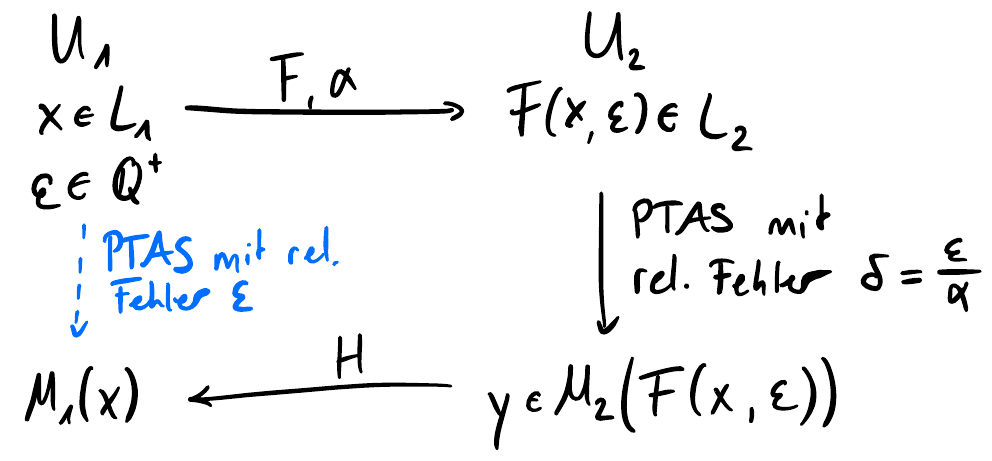
\includegraphics[width=0.4\textwidth]{images/ap-reduktionen.png}
    \caption{AP-Reduktionen}
\end{figure}

\paragraph{Lemma}
Seien $U_1, U_2$ Optimierungsprobleme wie oben.
Falls $U_1 \leq_{AP} U_2$, so gilt:
$$ \exists \text{ PTAS für } U_2 \implies \exists \text{ PTAS für } U_1 $$
$$ \not \exists \text{ PTAS für } U_1 \implies \not \exists \text{ PTAS für } U_2 $$

\underline{Beweis}: offensichtlich. Siehe Buch S.320.

\paragraph{APX-vollständig}
Ein Problem $U \in NPO$ heisst \emph{APX-vollständig (APX-complete)} falls gilt:
\begin{enumerate}
    \item $U \in APX$
    \item $\forall W \in APX \cl W \leq_{AP} U$
\end{enumerate}

\paragraph{Max-SAT}
Eingabe: Formel $C = C_1 \wedge ... \wedge C_m$ in KNF über Variablen $x_1, ..., x_n$.
Ziel: Belegung die die Anzahl erfüllter Klauseln maximiert.

\paragraph{Max-CLIQUE (Max-CL)}
Eingabe: ungerichteter Graph $G$.
Ziel: Clique in $G$ mit maximaler Knotenanzahl.

\paragraph{Lemma}
Max-SAT $\leq_{AP}$ Max-CLIQUE

\underline{Beweis:} Konstruktion (sei $C_i = l_{i1} \vee ... \vee l_{ij_i}$):
\begin{itemize}
    \item $\alpha = 1$
    \item $ F(C, \varepsilon) = F(C) = G_C = (V,E) $ mit
        $ V = \{ (i, k) \st 1 \leq i \leq m \; , \; 1 \leq k \leq j_i \}$
        (jede occurence eines Literals hat einen Knoten) und
        $ E = \{ \{ (r,s) , (p,q) \} \st r \neq p \; , \; l_{rs} \not \equiv \overline{l}_{pq} \} $
        (keine Kanten innerhalb einer Klausel, und keine Widersprüche)
        \footnote{D.h. $F$ ist unabhängig von $\varepsilon$.}
    \item $ H $ wählt eine Belegung $\gamma$ wie folgt:
        für die Literale in der gefundenen Max-Clique, wähle $x_i=1$ und $\overline{x}_i=0$.
        Wähle alle anderen Literale beliebig.
\end{itemize}
Dies erfüllt unsere Bedingungen:
(i) Eingabe wird gemapped. (ii) Ausgabe wird gemapped.
(iii) $F, H$ in Polynomzeit berechenbar. (iv) $F, H$ unabhängig von $\varepsilon$.
(v) Jede Clique $Q$ der Grösse $q$ erfüllt $\geq q$ Klauseln.
Jede Belegung die $r$ Klauseln erfüllt, bestimmt eine Clique der Grösse genau $r$.
\\
$\implies cost_{Max-SAT}(H(G_C)) \geq cost_{Max-CLIQUE}(Q)$.

\begin{figure}[h]
    \centering
    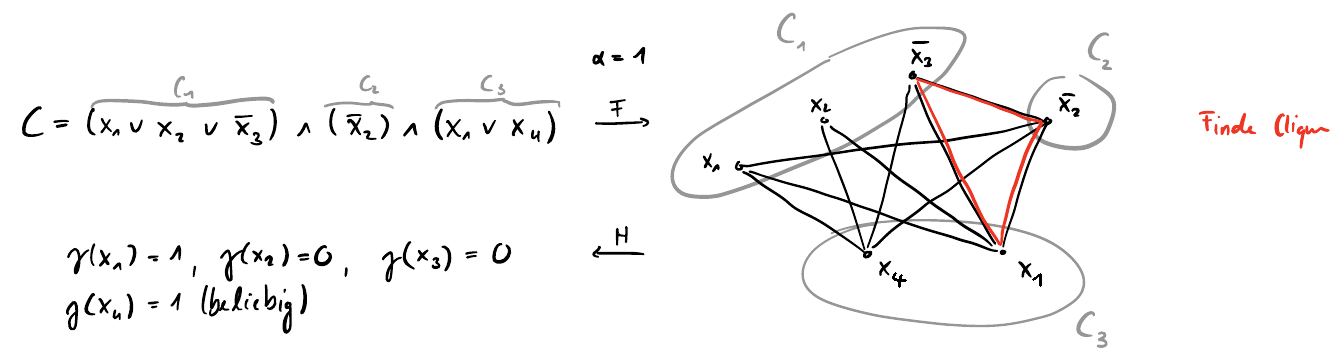
\includegraphics[width=0.8\textwidth]{images/ap-reduktion-beispiel.png}
    \caption{Beispiel AP-Reduktion Max-SAT $\leq_{AP}$ Max-CLIQUE}
\end{figure}

\paragraph{Fazit}
AP-Reduktionen sind intuitiv, aber in der Praxis schwer zu finden.

\newpage
\subsection{Lückenerhaltende Reduktionen (GP-Reduktionen)}

\paragraph{Schwellwertproblem}
Liegt die optimale Lösung oberhalb oder unterhalb des Schwellwerts $t$?

\paragraph{Lückenproblem}
Liegt die optimale Lösung oberhalb oder unterhalb der Lücke $[s,c)$? D.h. ist $Opt < s \vee Opt \geq c$?
Falls Lösung in der Lücke: keine Aussage.

Siehe \emph{Promise-Problem}: Es ist garantiert dass die Eingabe nicht $Opt \in [s, c)$ hat.

\underline{Fallunterscheidung:} Sei $y$ die berechenbar Lösung.
TODO drawings
\begin{itemize}
    \item Fall 1: $y \geq c$ (oberhalb):
        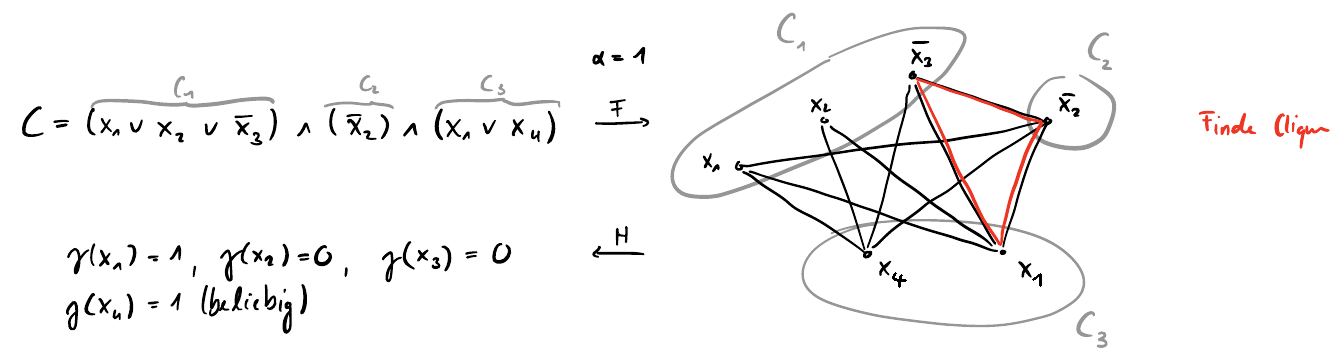
\includegraphics[width=0.2\textwidth]{images/ap-reduktion-beispiel.png}
        $\implies$ $Opt$ muss oberhalb liegen.
    \item Fall 2: $y < s$ (unterhalb):
        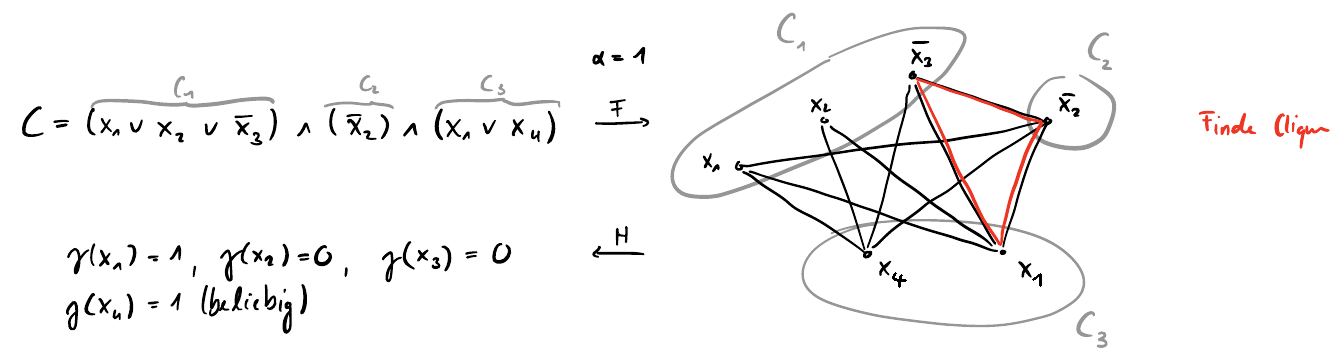
\includegraphics[width=0.2\textwidth]{images/ap-reduktion-beispiel.png}
        $\implies$ $Opt$ muss unterhalb liegen. \\
        Annahme: Approximation ist gut genug, so dass sie nicht über die Lücke geht.
    \item Fall 3: $y \geq s$ (innerhalb):
        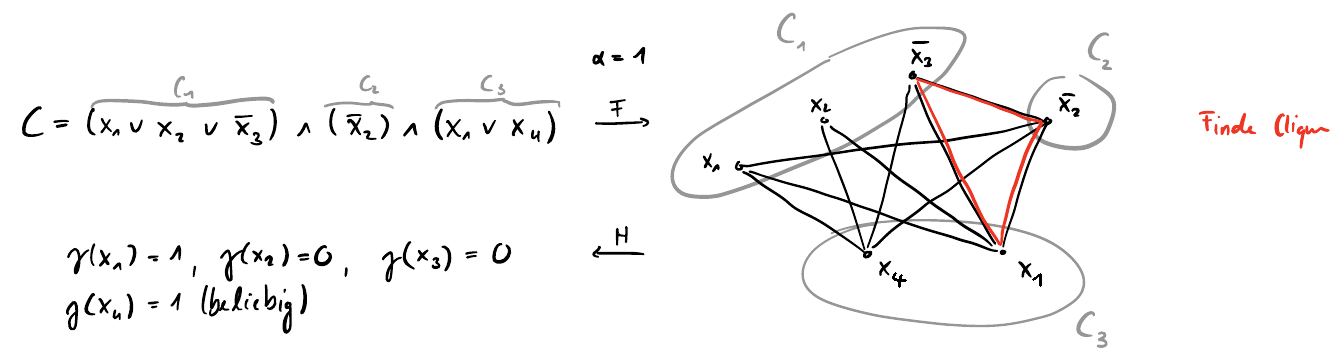
\includegraphics[width=0.2\textwidth]{images/ap-reduktion-beispiel.png}
        $\implies$ $Opt$ muss oberhalb liegen (kann nicht in der Lücke liegen).
\end{itemize}
In allen Fällen ist das Lückenproblem entscheidbar.
%
\begin{center}
    $\exists$ gute Approximation (kleine Lücke möglich) $\implies$ Lückenproblem entscheidbar

    Lückenproblem schwer $\implies$ $\not \exists$ gute Approximation
\end{center}
%
Beispiel:
Max-SAT ist selbst bei Lücke $ [s,c) = \left[ \frac{7}{8}, 1 \right) $ noch schwer.

\paragraph{Definition Lückenproblem GAP}
Sei $s, c\in \R^+, 0 \leq s \leq c \leq 1$.\footnote{Wir normalisieren auf $[0,1]$, siehe auch $|x|$ unten.}
Sei $U = (L, M, cost, goal) \in NPO$.
Das Lückenproblem $GAP_{s,c}(U)$ ist folgendes Entscheidungsproblem:

Eingabe:
$x \in L$ so dass $\frac{Opt_U(x)}{|x|} < s$ oder $\frac{Opt_U(x)}{|x|} \geq c$.
\\
Ausgabe:
JA, falls $\frac{Opt_U(x)}{|x|} \geq c$, sonst NEIN.

\paragraph{Lemma}
$GAP_{s,c}(U)$ NP-schwer ist $\implies$ $\not \exists$ polyzeit $\frac{c}{s}$-Approximation
für $U$ (falls P $\neq$ NP).

\underline{Beweis:}
Per Widerspruch. Nehme an es gäbe einen polyzeit $\frac{c}{s}$-Approximationsalgorithmus $A$.
OBdA sei $U$ ein Maximierungsproblem.
Zeige dass gilt:
$$ cost(A(x)) < s \cdot |x| \iff Opt_U(x) < s \cdot |x| $$
%
"$\Leftarrow$" : offensichtlich da $cost(A(x)) \leq Opt_U(x)$.

"$\Rightarrow$" : Nehme (für Widerspruch) an dass $Opt_U(x) \geq s \cdot |x|$.
Da die Lücke leer sein muss, gilt also $Opt_U(x) \geq c \cdot |x|$.
Ausserdem gilt per Definition von $\frac{c}{s}$-Approximation
$\frac{Opt_U(x)}{cost(A(x))} \leq \frac{c}{s}$.
Nun folgt ein Widerspruch:
$$ cost(A(x)) \geq \frac{s}{c} \cdot Opt_U(x) \geq \frac{s}{c} \cdot c \cdot |x| \geq s \cdot |x| $$

$\implies$ mit $A$ lässt sich $GAP_{s,c}(U)$ entscheiden. Widerspruch zu NP-schwer!

\paragraph{GP-Reduktion}
Seien $U_1, U_2$ Maximierungsprobleme.
Eine \emph{Lückenerhaltende Reduktion (gap-preserving reduction, GP-Reduktion)}
von $U_1$ zu $U_2$ mit Parametern $(s,c)$ und $(s',c')$ ist ein polyzeit Algorithmus $A$ mit:
\begin{enumerate}[label=(\roman*)]
    \item $ \forall x\in L_1 \cl A(x) \in L_2 $
    \item $ \frac{Opt_{U_1}(x)}{|x|} \geq c \implies \frac{Opt_{U_2}(A(x))}{|A(x)|} \geq c' $
    \item $ \frac{Opt_{U_1}(x)}{|x|} < s \implies \frac{Opt_{U_2}(A(x))}{|A(x)|} < s' $
\end{enumerate}

\underline{Bemerkung:}
Falls $\exists$ GP-Reduktion und $GAP_{s,c}(U_1)$ NP-schwer ist $\implies$ $GAP_{s',c'}(U_2)$ NP-schwer

$\implies$ untere Schranke $\frac{c}{s}$ für Approximation von $U_1$ $\implies$ untere Schranke
$\frac{c'}{s'}$ für Approx. von $U_2$

\underline{Motivation:} GP-Reduktion ist simpler als AP-Reduktion (nur ein Algorithmus).

\paragraph{Beispiel (MAX-E3SAT, MAX-2SAT)}
Eingabe: KNF-Formel. Ziel: Belegung finden die alle/möglichst viele Klauseln erfüllt.
\begin{itemize}
    \item \textbf{E3SAT}: exakt 3 verschiedene Literale pro Klausel
    \item \textbf{2SAT}: $\leq 2$ Literale pro Klausel, in P
    \item \textbf{MAX-2SAT}: NP-schwer
\end{itemize}

\paragraph{Lemma}
Für alle $a,b, \; a \neq 0, a \leq b$ existiert eine GP-Reduktion von MAX-E3SAT auf MAX-2SAT
mit Parametern $(a,b)$ und $\left( \frac{3}{5} + \frac{a}{10} , \frac{3}{5} + \frac{b}{10} \right)$.
\footnote{D.h. die Lücke/Approximation wird etwas schlechter.}

\underline{Beweis:}
Sei $C = C_1 \wedge ... \wedge C_m$ eine MAX-E3SAT-Instanz mit Klauseln
$C_i = l_{i1} \vee l_{i2} \vee l_{i3}$ und Variablen $x_1, ..., x_n$.

Konstruiere MAX-2SAT-Instanz: $\Phi_C = \bigwedge_{i=1}^m \Phi(C_i)$ mit zusätzlichen Variablen
$y_1, ..., y_m$ und mit
\begin{align*}
\Phi(C_i) &= (l_{i1}) \wedge (l_{i2}) \wedge (l_{i3}) \\
    & \wedge (\overline{l_{i1}} \vee \overline{l_{i2}}) \wedge (\overline{l_{i1}} \vee \overline{l_{i3}}) \wedge (\overline{l_{i2}} \vee \overline{l_{i3}}) \\
    & \wedge (l_{i1} \vee \overline{y_i}) \wedge (l_{i2} \vee \overline{y_i}) \wedge (l_{i3} \vee \overline{y_i}) \\
    & \wedge (y_i)
\end{align*}

Restlicher Beweis siehe Buch S.327.
Idee: für jede Belegung $\alpha$ für $C$ kann man $y_i$ so wählen dass $\leq 7$ der 10 Klauseln
erfüllt werden.

\paragraph{Lemma (Max-CLIQUE)}
Max-CLIQUE kann GP-reduziert werden auf Max-CLIQUE mit Parametern
$(\alpha, 1-\varepsilon), \; (\alpha^2, (1-\varepsilon)^2)$
für alle $\alpha \in (0, 1-\varepsilon), \; \varepsilon \in (0, \frac{1}{2})$.

\underline{Beweis:}
Sei $G=(V,E), \; |G|=|V|$.
Konstruiere $G \times G = ( V_{G \times G}, E_{G \times G} )$ mit
\begin{itemize}
    \item $V_{G \times G} = V \times V$
    \item $E_{G \times G} = \left\{ \{ (v,u) , (r,s) \} \st v,u,r,s \in V \text{ und }
    ( ( v=r , \{u,s\} \in E) \text{ oder } (\{v,r\} \in E) ) \right\}$
\end{itemize}

$Opt_{Max-CLIQUE}(G)$ = Clique der Grösse $k$ in $G$ $\implies$ Clique der Grösse $k^2$ in $G \times G$.

Fallunterscheidung:
\begin{itemize}
    \item $ Opt_{Max-CLIQUE}(G) < a \cdot |G| \implies
        Opt_{Max-CLIQUE}(G \times G) < a^2 \cdot |G|^2 = a^2 \cdot |G \times G|$
    \item $ Opt_{Max-CLIQUE}(G) \geq (1-\varepsilon) \cdot |G| \implies
        Opt_{Max-CLIQUE}(G \times G) \geq (1-\varepsilon)^2 \cdot |G|^2 = (1-\varepsilon)^2 \cdot |G \times G|$
\end{itemize}

\underline{Implikation:}

Jede konstante $c$-Approximation lässt sich iterativ verbessern (von $c$ auf $\sqrt{c}$, für $c>1$). \\
$\implies$ \emph{entweder} Max-CLIQUE $\in$ PTAS \emph{oder} Max-CLIQUE $\noindent$ APX
(= nicht konstant approximierbar).

Max-SAT $\leq_{AP}$ Max-CLIQUE (siehe \autoref{sec:ap-reduktionen}) und Max-SAT ist APX-vollständig
\footnote{Nicht in Vorlesung bewiesen} \\
$\implies$ Max-CLIQUE $\notin$ APX

TODO Beispiel Graphik

\newpage


\part{Online-Algorithmen}

\section{Einführung und das Paging-Problem}

\begin{takeaway}
    \item Online-Problem, Online-Algorithmus, kompetitiver Faktor
    \item Skirental-Problem
    \item Paging-Problem
    \item Randomisierte Online-Algorithmen
    \item Yaos Prinzip
\end{takeaway}

\paragraph{Motivation}
Probleme lösen und Entscheidungen fällen ohne alle für eine optimale Lösung relevanten Informationen zu haben.
Stattdessen werden die Informationen stückweise zur Laufzeit bekannt.

\paragraph{Beispiel: Skirental-Problem}
Unendlich langer Urlaub, nur an schönen Tagen Ski fahren.
Skier mieten für 1 CHF pro Tag, oder kaufen für $k$ CHF.
Erst am Tag selbst wird bekannt ob ein Tag schön ist.

Optimale Lösung: Sei $s$ die Anzahl schöner Tag.
Miete bei $s < k$, kaufe bei $s > k$, bei $s=k$ egal.

Problem: $s$ nicht bekannt, erst am Tag selber wird bekannt ob ein Tag schön ist.

\begin{table}[h]
    \begin{tabular}{l|l|c}
        Szenario & Worst Case & Approximationsgüte \\ \hline
        An Tag 1 kaufen & Ab Tag 2 schlechtes Wetter & $\frac{k}{1}$ \\
        Immer mieten & An $x >> k$ Tagen schönes Wetter & $\frac{x}{k}$ \\
        An $k-1$ Tagen mieten, an Tag $k$ kaufen & Ab Tag $k+1$ schlechtes Wetter & $\frac{2k-1}{k} = 2-\frac{1}{k}$
    \end{tabular}
\end{table}
\begin{figure}[h]
    \centering
    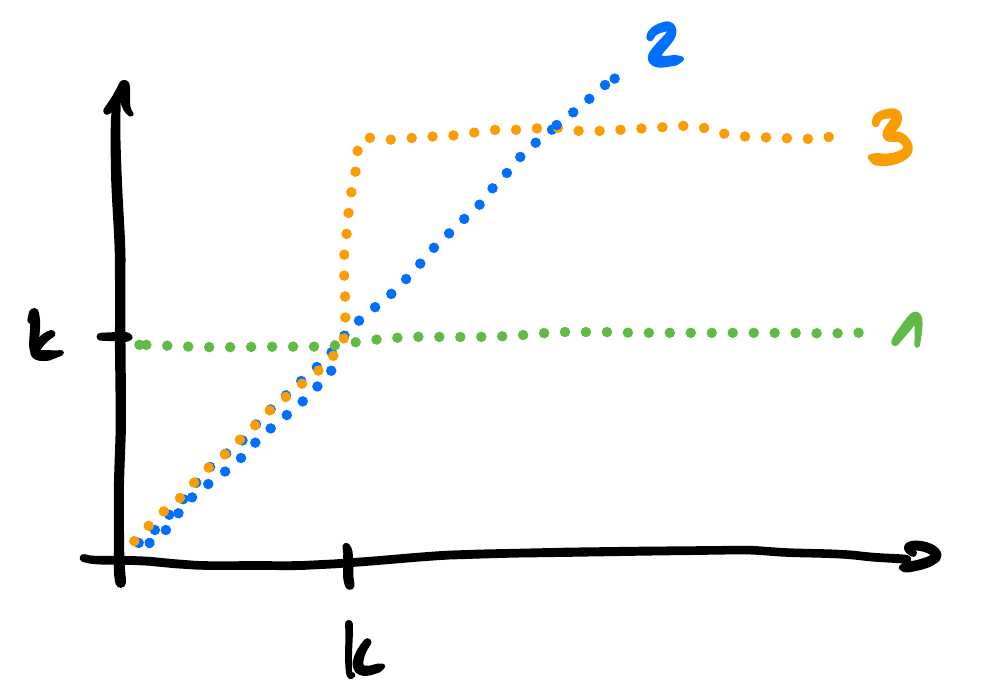
\includegraphics[width=0.3\textwidth]{images/skirental.png}
    \caption{Skirental Szenarios}
\end{figure}

\paragraph{Online-Problem}
Ein \emph{Online-Minimierungsproblem} ist $\Pi = (I, O, cost, \min)$.
Eine Eingabe $I = (x_1, ..., x_n) \in \mathcal{I}$ ist eine Folge von \emph{Anfragen},
jeweils für \emph{Zeitschritt} $i$.
Eine akzeptierte Lösung $O = (y_1, ..., y_n)$ ist eine Folge von \emph{Antworten}.

Beim analogen Maximierungsproblem spricht man statt von $cost(I, O)$ oft vom \emph{Gewinn} $gain(I,O)$.

\paragraph{Online-Algorithmus}
Sei $\Pi$ ein Online-Optimierungsproblem.
Ein \emph{Online-Algorithmus} $\A$ berechnet die Ausgabe $\A(I) = (y_1, ..., y_n) $
wobei $y_i$ nur von $(x_1, ..., x_i)$ abhängt.
$\A(I)$ ist eine zulässig Lösung für $I$.

\paragraph{Kompetitiver Faktor}
(aka. competitive ratio, Wettbewerbsgüte, kompetitive Güte) \\
Ein Online-Algorithmus $\A$ ist \emph{c-kompetitiv} falls gilt:
\begin{align*}
\exists \alpha \geq 0 \quad \forall I \cl \quad cost(\A(I)) & \leq c \cdot cost(Opt(I)) + \alpha \\
\dfrac{cost(\A(I))}{cost(Opt(I))} + \alpha' & \leq c
\end{align*}
für ein Minimierungsproblem und $\alpha$ konstant.
$Opt$ ist ein optimaler Offline-Algorithmus, d.h. mit vollständiger Information.

Für Maximierungsprobleme:
$$ gain(Opt(I)) \leq c \cdot gain(\A(I)) + \alpha $$

Das kleinste $c$ für das dies gilt heisst \emph{kompetitiver Faktor}. \\
$\A$ heisst \emph{strikt c-kompetitiv} falls $\alpha = 0$. \\
$\A$ heisst \emph{optimal} falls er strikt 1-kompetitiv ist ($\alpha = 0, c = 1$).

Wir sprechen hierbei von \emph{kompetitiver Analyse}.
Der kompetitiver Faktor ist vergleichbar mit der Approximationsgüte von Approximationsalgorithmen.

Ein Online-Algorithmus heisst \emph{kompetitiv} wenn sein kompetitiver Faktor nicht von der
Länge der Eingabe abhängt (d.h. es keine Startkosten gibt die amortisiert werden müssen).
Die Konstante $\alpha$ ist wichtig da sie erlaubt auf kurze Eingaben schlecht zu sein
(und erst auf lange besser zu werden).
\footnote{Warum brauchen wir bei der Approximationsgüte keine vergleichbare Konstante?}

\paragraph{Untere Schranken beweisen}
Für einen strikt kompetitiven Algorithmus:
Finde eine Instanz $I$ mit $\frac{\A(I)}{Opt(I)} > c$ $\implies$ \underline{nicht} strikt-kompetitiv.

Für einen nicht-strikt kompetitiven Algorithmus:
Finde eine unendliche Folge $I_1, I_2, ...$ von Instanzen so dass $\frac{\A(I_i)}{Opt(I_i)} > c$
und $Opt(I_i) \overset{i \rightarrow \infty}{\longrightarrow} \infty $.

\begin{figure}[h]
    \centering
    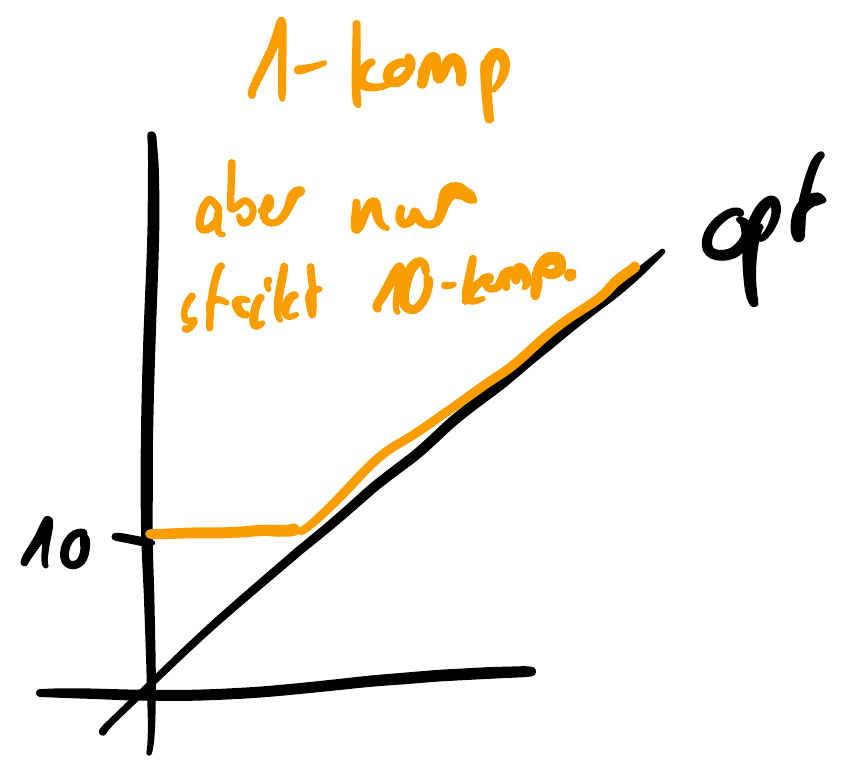
\includegraphics[width=0.2\textwidth]{images/strikt-kompetitiv.png}
    \caption{$Opt$ in schwarz. $\A$ in orange, 1-kompetitiv und strikt-10-kompetitiv.}
\end{figure}


\subsection{Das Paging-Problem}

\paragraph{Paging}
\begin{itemize}
    \item Eingabe: $ I = (x_1, ..., x_n)$ mit Speicher-Indizes $x_i \in \N$
    \item Hauptspeicher mit $m$ Seiten: $ (s_1, ..., s_m) $
    \item Cache-Speicher mit $k$ Seiten: $ B = (s_{j_1}, ..., s_{j_k}) $, initialisiert mit $ (s_1, ..., s_k) $
        \footnote{Der Vorsprung eines selbstgewählten Startinhalts kann in $\alpha$ versteckt werden.}
    \item Zeitschritt $i$:
    \begin{itemize}
        \item Index $x_i$ wird angefragt
        \item Falls $x_i$ im Cache (d.h. $s_{x_i} \in B$): return $y_i=0$
        \item Andernfalls: return $y_i=j$, und setze $B = B \backslash  \{s_j\} \cup \{s_{x_i}\} $,
            d.h. lösche Seite $s_j$ aus dem Cache und ersetze sie durch $s_{x_i}$.
            \footnote{Zusätzliches, proaktives Entfernen bringt keinen Vorteil.}
    \end{itemize}
    \item $ cost(\A(I)) := \vert \{ i \st y_i > 0 \} \vert $
    \item goal := min
\end{itemize}

Strategien bei \emph{Seitenfehlern (page faults)} zum \emph{Verdrängen} von Seiten:
First-in-First-Out (FIFO, wie eine Queue),
Last-in-First-Out (LIFO, wie ein Stack),
Least-Recently-Used (LRU),
Longest-Forward-Distance (LFD, offline-only!).

\paragraph{Satz (FIFO)}
Ein Online-Algorithmus für Paging der FIFO nutzt ist strikt-k-kompetitiv.

\underline{Beweis:}
Gruppiere Zeitschritte in \emph{Phasen}.
Phase 1 endet nach dem ersten Seitenfehler.
Phase $P \geq 2$ endet nach $1+ (P-1)k$ Seitenfehlern, d.h. alle $k$ Fehler endet eine Phase und beginnt eine neue.

In Phase 1 machen $Opt$ und $Fifo$ je genau einen Fehler (warum?).

Sei $s$ die Seite die den letzten Seitenfehler von Phase $P-1$ verursacht
(d.h. sie kommt neu in den Cache, und wird dank FIFO als letztes in Phase $P$ verdrängt werden). \\
$\implies$ Zu Beginn von Phase $P$ ist $s$ im Cache von $Opt$ \underline{und} von $Fifo$. \\
$\implies$ Es gibt $\leq k-1$ Seiten die im Cache von $Opt$ sind, aber nicht in dem von $Fifo$. \\
Während Phase $P$ macht $Fifo$ genau $k$ Fehler. \\
$\implies$  Während $P$ muss $Opt$ mindestens einen Seitenfehler machen. \\
$\implies$  $Fifo$ ist k-kompetitiv.

LRU ist in der Theorie ebenfalls k-kompetitiv, in der Praxis allerdings tendenziell besser als FIFO.

\paragraph{Satz (untere Schranke)}
Kein Online-Algorithmus für Paging kann eine besseren kompetitiven Faktor als k erreichen.

\underline{Beweis:}
Sei $k$ die Grösse vom Cache und $k+1$ die Grösse vom Hauptspeicher.
\footnote{$k+1$ macht die Aussage nur stärker. Warum?}
Betrachte die "worst case" Eingabe $ I = (k+1, s_{y_1}, s_{y_2},, ..., s_{y_{n-1}}) $,
d.h. in Zeitschritt $i$ wird die Seite angefragt die $\A$ zuvor erst verdrängt hat.
$\A$ verursacht also exakt $k$ Seitenfehler, und $Opt$ nur einen in Zeitschritt 1.

\underline{Für alle Strategien} von $\A$ lässt sich eine worst-case Eingabe konstruieren (siehe Idee
eines \emph{Gegenspielers} der die Strategie/den Quellcode kennt).
Durch Wiederholen solcher k-langen Phasen lässt sich ausserdem eine \underline{unendlich lange}
Eingabe konstruieren.
Eingabelänge $n$, $\A$ mit $n$ Fehlern, $Opt$ mit $n/k$ Fehlern $\implies$ k-kompetitiv.
\footnote{Mit etwas Glück (abhängig davon was $\A$ in zukünftigen Phasen verdrängt)
macht $Opt$ sogar nur den Fehler in Zeitschritt 1, und macht danach nie wieder einen Fehler.}


\subsection{Randomisierte Online-Algorithmen}

\paragraph{Motivation}
Randomisierung verunmöglicht es dem Gegenspieler die genaue Strategie von $\A$ zu kennen,
d.h. es verunmöglicht ihm eine worst case Instanz zu konstruieren.

\paragraph{Randomisierter Online-Algorithmus}
Bekommt als Eingabe zusätzlich ein unendliche langes Zufallsband $\phi$ mit Zufallsbits
(die u.a.r. 0 oder 1 sind).
Jede Antwort $y_i$ darf nur von $ \phi, x_1, ..., x_i, y_1, ..., y_{i-1} $ abhängen.

\underline{Beobachtung:}
Jeder randomisierte Algorithmus $Rand$ der $b(n)$ Zufallsbits für Eingaben der Länge $n$ liest
kann als eine Menge $ strat(Rand) = \{ A_1, ..., A_{2^{b(n)}} \} $ von $2^{b(n)}$ deterministischen
Online-Algorithmen angesehen werden, von denen einer mit Wahrscheinlichkeit jeweils $\frac{1}{2^{b(n)}}$
ausgewählt wird.

\paragraph{Erwarteter kompetitiver Faktor}
Ein Online-Algorithmus $Rand$ ist \emph{c-kompetitiv im Erwartungswert} falls
$$ \exists \alpha \geq 0 \quad \forall I \cl \quad
\mathbb{E} [ cost(Rand(I)) ] \leq c \cdot cost(Opt(I)) + \alpha $$

Das kleinste $c$ für das dies gilt heisst \emph{erwarteter kompetitiver Faktor}. \\
$Rand$ heisst \emph{strikt c-kompetitiv im Erwartungswert} falls $\alpha = 0$.

\paragraph{Wahrscheinlichkeitsverstärkung}
Einen randomisierten Offline-Algorithmus der mit Wahrscheinlichkeit $\frac{1}{2}$ korrekt ist,
kann man $k$ Mal wiederholen um $\frac{1}{2^k}$ zu erreichen.
Online ist dies \underline{nicht} möglich, da wir direkt eine Antwort auf jede Anfrage geben müssen.

\paragraph{Randomisierter Paging-Algorithmus RMark}
Eine Phase endet/beginnt wenn nach einem Seitenfehler alle Seiten unmarkiert werden.

\begin{algorithm}[h]
\caption{RMark}
\begin{algorithmic}
    \State mark alle Seiten im Cache
    \While{Eingabe ist noch nicht beendet}
        \State $s \gets$ Seite mit Index $x_i$
        \If{$s$ ist im Cache}
            \If{$s$ ist unmarkiert}
                \State mark $s$
            \EndIf
        \State output "0"
        \Else
            \If{es existiert keine unmarkierte Seite mehr im Cache}
                \State unmark alle Seiten im Cache
            \EndIf
            \State $s' \gets$ zufällig gewählte unmarkierte Seite
            \State verdränge $s'$ und füge $s$ an der alten Stelle von $s'$ ein
            \State mark $s$
            \State output "Index von $s'$ "
        \EndIf
    \State $i \gets i + 1$
    \EndWhile
\end{algorithmic}
\end{algorithm}


\paragraph{Satz}
$RMark$ hat einen erwarteten kompetitiven Faktor von $2 H_k$.
\footnote{Für jedes $l \in \N^+$ heisst $H_l$ die \emph{l-te Harmonische Zahl}
und $H_l := 1 + \frac{1}{2} + \frac{1}{3} + \dots + \frac{1}{l} = \sum_{i=1}^l \frac{1}{i} $.}
D.h. $RMark$ ist im Erwartungswert $\bigO(\log k)$-kompetitiv.

\underline{Beweis:} Siehe auch Skript S.14ff.

Betrachte eine einzelne Phase $P$.
O.B.d.A werden $k$ veschiedene Seiten angefragt (eventuell auch mehrmals).
Im worst case werden zuerst $l$ "neue" Seiten angefragt, und danach $k-l$ "alte".
Mit Wahrscheinlichkeit $(k-l)/k$ ist die erste alte Seite noch im Cache,
dann mit Wahrscheinlichkeit $(k-l-1)/(k-1)$ die zweite alte, usw.
Umgekehrt ist die $i$-te alte Seite mit Wahrscheinlichkeit
$1 - \frac{k-l-(i-1)}{k-(i-1)} = \frac{l}{k-(i-1)}$ \underline{nicht} mehr im Cache.
Die erwarteten Kosten während $P$ sind also
$$ l + \sum_{i=1}^{k-l} \dfrac{l}{k-(i-1)} = \dots = l (H_k - H_l +1) \leq l H_k $$
Ausserdem gilt $l \geq 1$ da jede Phase per Definition mit einer neuen Seite beginnt.

Betrachte die Kosten von $Opt$.
Betrachte zwei aufeinanderfolgende Phasen $P_{j-1}, P_j$.
In diesen wurden $\geq k+l_j$ verschiedene Seiten angefragt.
$\implies$ $Opt$ macht $\geq l_j$ Seitenfehler.
$RMark$ und $Opt$ machen in $P_1$ beide $l_1$ Fehler (da sie mit demselben Cache starten).

Durch unterschiedliches Gruppieren ($(P_1, P_2), (P_3, P_4), ...$ vs $P_1, (P_2, P_3), (P_4, P_5), ...$)
erhalten wir:
$$ cost(Opt(I))
    \geq \max \left\{ \sum_{i=1}^{ \lfloor N/2 \rfloor } l_{2i} , \sum_{i=1}^{ \lceil N/2 \rceil } l_{2i-1} \right\}
    \geq \frac{1}{2} \left( \sum_{i=1}^{ \lfloor N/2 \rfloor } l_{2i} + \sum_{i=1}^{ \lceil N/2 \rceil } l_{2i-1} \right)
    = \sum_{i=1}^{N} \frac{1}{2} l_i
$$

Der kompetitive Faktor ist also
$$ c \geq \dfrac{ \sum_{i=1}^{N} H_k l_i }{ \sum_{i=1}^{N} \frac{1}{2} l_i } = 2 H_k $$

\paragraph{Verbesserung}
Für Paging existiert kein deterministischer Online-Algorithmus mit kompetitivem Faktor $k$ (s.o.).
Mit Randomisierung können wir im Erwartungswert aber $\bigO(\log k)$ erreichen!
D.h. asymptotisch expontentieller Speedup!
Dies ist asymptotisch optimal für randomisierte Algorithmen (s.u.).


\subsection{Yaos Prinzip}

\paragraph{Motivation}
Untere Schranke für kompetitiven Faktor von deterministischen OAs
$\implies$ Untere Schranke für erwarteten kompetitiven Faktor von randomisierten OAs

Wahrscheinlichkeitsverteilung über Instanzen $\Pr_{Adv}$ $\implies$ W'keitsverteilung über Algorithmen $\Pr_{Rand}$.

Limitierung: konstante Anzahl von Instanzen $\I = \{I_1, ..., I_m\}$ und Algorithmen
$strat(Rand) = \{A_1, ..., A_l\}$ (d.h. Eingabelänge $n$ begrenzt).

\paragraph{Lemma 1 (1.13)}
Sei $\Pi$ ein Optimierungsproblem, sei $\I$ eine Klasse von Instanzen.
Sei $\Pr_{Adv}$ eine W'keitsverteilung so dass gilt:
$$ \forall A \in strat(Rand) \cl \E_{Adv}[cost(A(\mathsf{I}))] \geq c \cdot \E_{Adv}[cost(Opt(\mathsf{I}))] $$
Dann gilt:
$$ \forall Rand \; \exists I \in \I \cl \E_{Rand}[cost(\mathsf{A}(I)))] \geq c \cdot cost(Opt(I)) $$
wobei $\mathsf{A} ,\mathsf{I}$ Zufallsvariablen sind aus den Wahrscheinlichkeitsräumen $\Pr_{Rand}, \Pr_{Adv}$.

\underline{Beweis:} Siehe Skript S.18f.

\paragraph{Lemma 2 (1.14)}
Seien $\Pi, \I, \Pr_{Adv}$ wie oben.
Sei $\forall$ det. OAs $A_j$ der erwartete kompetitive Faktor $\geq c$, d.h.
$$ \E_{Adv} \left[ \dfrac{cost(A_j(\mathsf{I}))}{cost(Opt(\mathsf{I}))} \right] \geq c $$

Dann gilt:
$\forall$ rand. OAs ist der erwartete kompetitive Faktor $\geq c$, d.h. $\exists I \in \I$ so dass
$$ \dfrac{ \E_{Rand} [ cost(\mathsf{A}(I)) ]}{cost(Opt(I))} \geq c $$

\underline{Beweis:} Siehe Skript S.20f.

\paragraph{Satz (Yaos Prinzip)}
Folgt aus Lemma 1 und 2.
Seien $\Pi, \I, \Pr_{Adv}$ wie oben.
Für jeden randomisierten Online-Algorithmus existiert dann eine Eingabe $I$ so dass
$$
\dfrac{\E_{Rand}[cost(\mathsf{A}(I))]}{cost(Opt(I))}
    \geq \max \left\lbrace
    \left\lbrace \min_j \dfrac{\E_{Adv}[cost(A_j(\mathsf{I}))]}{\E_{Adv}[cost(Opt(\mathsf{I}))]} \right\rbrace,
    \left\lbrace \min_j \E_{Adv} \left[ \dfrac{cost(A_j(\mathsf{I}))}{cost(Opt(\mathsf{I}))} \right] \right\rbrace
    \right\rbrace
$$

Anders formuliert (laut Wikipedia):
$$ \max_{I \in \I} \E_{Rand}[cost(\mathsf{A}(I))] \geq \min_{A \in strat(Rand)} \E_{Adv}[cost(A(\mathsf{I} ))] $$
wobei $\mathsf{A}, \mathsf{I}$ Zufallsvariablen sind.

\paragraph{Spieltheoretische Interpretation}
Yaos Minimax Prinzip. Spezialfall von Von Neumanns Minimax Theorem (in Nullsummenspielen mit
2 Spielern und gemischten Strategien gibt es ein Gleichgewicht).
Zero-sum game, Spieler A wählt den det. Algorithmus, Spieler B wählt die Instanz, der payoff ist $cost(A_j(I))$.

Für jeden Spieler ist "zufällig wählen" eine Strategie.
Aus Yao folgt: für eine fixe Eingabe zufällig eine Algo wählen ist nicht schlechter
als für einen fixen Algo zufällig eine Eingabe wählen.

\paragraph{Satz (Untere Schranke für randomisiertes Paging)}
Kein randomisierter Online-Algorithmus für Paging kann einen besseren (= kleineren) erwarteten
kompetitiven Faktor als $H_k$ erreichen.

\underline{Beweis:}
Siehe Skript S.27ff.

Analog zu Paging: $k$ Cache, $k+1$ Hauptspeicher, frage zuerst $s_{k+1}$ an, danach (neu!) jede
der nicht gerade angefragten Seiten mit Wahrscheinlichkeit $\frac{1}{k}$.
Eine Phase endet nach $k$ Fehlern, d.h. nachdem alle $k+1$ Seiten mind. einmal angefragt wurden.

Betrachte einzelne Phase. Zeige dass für alle deterministischen  $A_j$ die erwarteten Kosten circa
\mbox{$H_k$-mal} höher sind als die von $Opt$.
Es gilt für die Eingabe während Phase $P$:
$$ \dfrac{\E_{Adv} [cost(A_j(P))]}{\E_{Adv} [cost(Opt(P))]} \geq \dfrac{|P|\cdot \frac{1}{k}}{1} = \dfrac{|P|}{k} $$

Schätze ab (siehe Skript, siehe Coupon Collector): $\quad \E_{Adv}[\,|P|\,] = 1 + k \cdot H_k$.

Wende Yaos Prinzip an:
$$ \dfrac{\E_{Rand}[cost(\mathsf{A}(I))]}{cost(Opt(I))} \geq H_k $$

\newpage

\section{k-Server-Problem}

\begin{takeaway}
    \item k-Server-Problem
    \item Potentialfunktionen, amortisierte Kosten (Teleskopsumme)
    \item Greedy, Double Coverage (Alternating Moves)
\end{takeaway}

\paragraph{Motivation}
Bewege Objekte in einem Raum zu bestimmten Punkten.
Z.B. Polizisten von Dienststellen zu crime scenes, oder Taxis zu Kunden.

``Heiliger Gral'' der Online-Algorithmen, wie TSP für Approximations-Algorithmen oder SAT für NP.

\paragraph{Metrischer Raum}
Sei $S$ eine Menge von Punkten, sei $\dist : S \times S \mapsto \mathbb{R}$ eine Distanzfunktion.
$\mathcal{M}(S, \dist)$ ist ein \emph{metrischer Raum} falls gilt:
Definitheit, Symmetrie, Dreiecksungleichung.

Beispiel: Euklidischer Raum. Vollständige, gewichtete, ungerichtete Graphen mit Dreiecksungleichung.
\\
Beobachtung: Alle Graphen mit Kastenkosten $\in \{1, 2\}$ erfüllen die Dreiecksungleichung.

\paragraph{k-Server}
Sei $\mathcal{M}(S, \dist)$ ein metrischer Raum.
Sei $s_1, ..., s_k$ Server als Punkte in $S$.
Sei eine Multimenge $C_i \subseteq S$ mit $|C_i|=k$ eine \emph{Konfiguration} von Servern in Zeitschritt $i$.
\\
Die \emph{Distanz} \footnote{Achtung Verwechslungsgefahr!}
zwischen $C_r$ und $C_t$ sind die Kosten eines minimalen Matchings zwischen ihnen.

Eine Instanz $I = (x_1, ..., x_n)$ fragt Punkte an, so dass in Zeitschritt $i$ ein Server nach $x_i$
bewegt werden muss (falls dort noch keiner steht).

Ziel: $\min \sum_i costMinMatching(C_i, C_{i+1})$

\paragraph{Träge}
Ein Online-Algorithmus für k-Server heisst \emph{träge (lazy)} wenn er nur dann einen Server bewegt,
wenn auf $x_i$ noch kein Server steht.
Auch bewegt er pro Zeitschritt maximal einen Server.

Dies erleichtert die Analyse. Gleichzeitig gilt (Satz): \\
Jeder c-kompetitive OA für k-Server kann in einen trägen OA umgewandelt werden der auch c-kompetitiv ist.

\paragraph{k-Server als Verallgemeinerung von Paging}
Cache $k$, Hauptspeicher $m$ $\longrightarrow$ vollständiger Graph mit $m$ Knoten und initial
Servern auf $(v_1, ..., v_k)$. Angefragte Punkte = angefragte Seiten.

Daraus folgt eine untere Schranke (Satz):
Es existiert ein metrischer Raum so dass kein deterministischer OA für k-Server besser als k-kompetitiv ist.
\\
Frage: für Paging ist die Schranke scharf, d.h. wir kennen einen Algo (z.B. FIFO).
Können wir für k-Server auch einen Algo konstruieren?

\paragraph{k-Server Vermutung(en)}
\begin{itemize}
    \item Es existiert ein k-kompetitiver deterministischer OA für k-Server.
    \item Es existiert ein im Erwartungswert $\Theta(\log k)$-kompetitiver randomisierter OA für k-Server.
\end{itemize}
D.h. die untere Schranke ist erreichbar.
Wenn dies wahr ist, dann ist k-Server genauso schwer wie Paging!
Aktueller Stand: $2k-1$.

\paragraph{Greedy-Algorithmus}
Bewege immer den Server der am nähesten dran ist.

\underline{Satz:}
$Greedy$ ist nicht kompetitiv für k-Server.

\underline{Beweis:}
Siehe Instanz in \autoref{k-server-greedy}.
Hier gilt $\frac{cost(Greedy(I))}{cost(I)} = \frac{n}{2}$, d.h. es gibt keine Konstante $c$
so dass $Greedy$ $c$-kompetitiv wäre.

\begin{figure}[h]
    \centering
    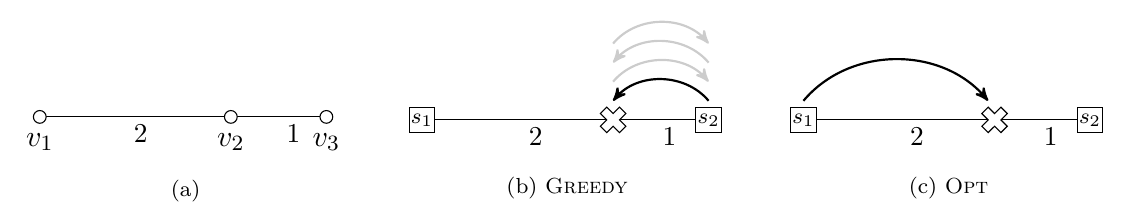
\includegraphics[width=0.8\textwidth]{images/k-server-greedy.png}
    \caption{k-Server: $Greedy$ versus $Opt$}
    \label{k-server-greedy}
\end{figure}


\subsection{Potentialfunktionen}

\paragraph{Motivation}
Kompetivität $c$ abschätzen über die \emph{amortisierten Kosten}.
Statt dass $cost(A(I)) \leq c \cdot cost(Opt(I)) + \alpha$ für alle $I$ gelten muss,
wollen wir zeigen dass $cost(A(x_i)) \leq c \cdot cost(Opt(x_i)) + \alpha$ für alle $x_i$ gilt.
\\
Dann können wir erlauben dass $A$ in einigen Zeitschritten mehr als $c$-mal schlechter ist als $Opt$,
solange er in anderen wieder weniger schlecht ist.

\paragraph{Potentialfunktion}
Sei $\mathcal{K}_{Alg}$ die Menge aller \emph{Konfigurationen} von $A$ auf Instanz $I$
und sei $\mathcal{K}_{Opt}$ die Menge aller Konfigurationen eines beliebigen, aber festen, $Opt$.
\footnote{Konfiguration: nach aussen sichtbar, nicht der interne state der Turingmaschine.
Z.B. Position der Server, Seiten im Cache.}

Dann ist eine \emph{Potentialfunktion} $\Phi$:
$$
\Phi \cl  \mathcal{K}_{Alg} \times \mathcal{K}_{Opt} \mapsto \R
\qquad \text{oder} \qquad
\Phi \cl \I \mapsto \R
$$
Die Konfigurationen sind eindeutig durch die Eingabe gegeben, daher die beiden Darstellungen.

Das \emph{Potential} in Zeitschritt $i$ ist $\Phi(x_i)$.

Die \emph{amortisierten Kosten} (vgl. \emph{tatsächliche Kosten}) sind:
$$ amcost(A(x_i)) := cost(A(x_i)) + \Phi(x_i) - \Phi(x_{i-1})$$

\paragraph{Satz}
Falls
$$ \exists \beta \in \R^+ \text{konstant} \; \forall i \in [1,n] \cl 0 \leq \Phi(x_i) \leq \beta
\quad \wedge \quad
amcost(A(x_i)) \leq c \cdot cost(Opt(x_i))
$$
dann ist $A$ $c$-kompetitiv für $\Pi$.

Dies lässt sich verallgemeinern dass $\Phi$ negativ werden darf, solange es trotzdem durch
eine Konstante beschränkt ist.

\underline{Beweis:}
Siehe Skript S.48. Kurz:
$$ cost(A(I)) = \sum_{i=1}^n cost(A(x_i)) = \dots \leq c \cdot cost(Opt(I)) + \beta $$
Amortisierte Kosten einsetzen, dann Potentiale auscanceln (\emph{Teleskopsumme}).
Dann $\alpha := \beta$ setzen.

\subsection{k-Server auf der Linie}

\paragraph{Die Line}
Betrachte den metrischen Raum $\M_{[0,1]} = ([0,1], \dist)$ mit $\dist(x,y) = |x-y|$,
d.h. den Zahlenstrahl der reellen Zahlen zwischen 0 und 1.

\paragraph{Double Coverage-Algorithmus}
Idee: bewege von beiden Seiten eine Server je um die selbe Distanz in Richtung $x_i$.
Nicht träge!

\begin{figure}[h]
    \centering
    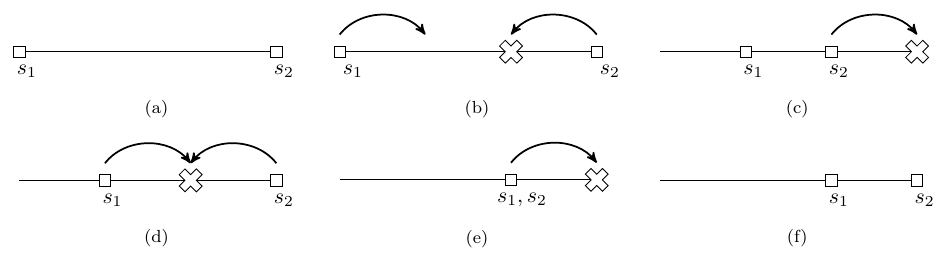
\includegraphics[width=0.8\textwidth]{images/k-server-double-coverage.png}
    \caption{k-Server: $DoubleCoverage$ anhand von $Greedys$ worst-case Beispiel}
    \label{k-server-double-coverage}
\end{figure}

\begin{algorithm}[h]
\caption{Double Coverage (ein Zeitschritt)}
\begin{algorithmic}
    \State $s \gets x_i$
    \State $s_{rechts} \gets \lambda; s_{links} \gets \lambda$
    \State $s_{rechts} \gets $ Server direkt rechts neben $s$
    \State $s_{links} \gets $ Server direkt links neben $s$
    \If{$s_{rechts} = \lambda$}
        \State output "Bewege $s_{links}$ zu $s$"
    \ElsIf{$s_{links} \gets \lambda$}
    \State output "Bewege $s_{rechts}$ zu $s$"
    \Else
    \State $d \gets \min \{ \dist(s_{rechts} , s), \dist(s_{links} , s) \}$
    \State output "Bewege $s_{rechts}$ um $d$ nach links und $s_{links}$ um d nach rechts"
    \EndIf
\end{algorithmic}
\end{algorithm}

\paragraph{Satz}
$DoubleCoverage$ ist k-kompetitiv für k-Server auf $\M_{[0,1]}$.

\underline{Beweis}:
Siehe Skript S.49ff.

Ziel: Definiere Potentialfunktion $\Phi$ so dass die Bedingungen vom Satz gelten.
\\
Sei $K_{DC} = \{p_1^{DC}, \dots , p_k^{DC}\}$ eine Konfigurationen von DC (d.h. die Positionen seiner Server).
Sei $K_{Opt}$ analog.
Seien $M_{\min} (K_{DC}, K_{Opt})$ die Kosten eines minimalen Matchings
und sei $DC(K_{DC})$ die Summe der paarweisen Distanzen aller Server von DC.
Wir definieren:
$$\Phi (K_{DC}, K_{Opt}) := k \cdot M_{\min} (K_{DC}, K_{Opt}) + DC(K_{DC}) $$

Beobachte: $\Phi$ ist positiv, konstant, und hängt nicht von $n$ ab. Konkret (Bedingung 1):
\footnote{Recall that wir uns in $\M_{[0,1]}$ bewegen, d.h. alle Distanzen zwischen zwei Punkten sind $\leq 1$.}
$$ 0 \leq \Phi (K_{DC}, K_{Opt}) \leq k \cdot k + \binom{k}{2} \leq 2 k^2 := \beta $$

Zeige nun dass $\forall i$ gilt $(\star)$:
$ \Phi(x_i) - \Phi(x_{i-1}) \leq k \cdot cost(Opt(x_i)) - cost (DC(x_i)) $ (Bedingung 2).
\\
Schätze dazu ab wie sich das Potential verändert (durch die Änderung der Konfiguration)
wenn erst $Opt$ und dann $DC$ einen Zug machen (\emph{Alternating Moves}).

Der Zug von $Opt$ vergrössert $\Phi$ um $\leq k \cdot cost(Opt(x_i))$
(maximal ein Server wird um $cost(Opt(x_i))$ bewegt, nur $k \cdot M_{\min}$ ist affected).

Der Zug von $DC$ verändert $\Phi$ um:
\begin{itemize}
    \item[Fall 1:] $x_i$ ist ``ganz aussen''. OBdA wird $s_{rechts}$ nach links verschoben.
        Der zweite Summand vergrössert das Potential um $\leq (k-1) \cdot cost(DC(x_i))$.
        \\
        OBdA existiert ein minimales Matching das $s$ (von $Opt$ bereits nach $x_i$ bewegt)
        und $s_{rechts}$ matched -- siehe Fallunterscheidung).
        D.h. die Kosten von $k \cdot M_{\min}$ verringern sich um $k \cdot cost(DC(x_i))$.
        \\
        $\implies$ insgesamt gilt $(\star)$
    \item[Fall 2:] $x_i$ ist zwischen $s_{links}$ und $s_{rechts}$.
        Der zweite Summand wird um $cost(DC(x_i))$ kleiner (da sich $s_{links}, s_{rechts}$ näher kommen).
        OBdA sind vor dem Zug von $DC$ $s$ und $s_{links}$ (oder $s$ und $s_{rechts}$) gematched.
        Dies verringert die Kosten von $M_{\min}$ um $cost(DC(x_i))/2$.
        \\
        Der andere wird mit einem $s'''$ von $Opt$ gematched.
        Hier erhöhen sich die Kosten um $\leq cost(DC(x_i))/2$.
        D.h. der erste Summand bleibt gleich oder wird kleiner.
        \\
        $\implies$ insgesamt gilt $(\star)$
\end{itemize}
$\implies$ Bedingung 1 + 2 vom Satz erfüllt $\implies$ $DC$ ist k-kompetitiv.

\newpage

\section{Advice-Komplexität}

\begin{takeaway}
    \item Advice-Komplexität, Online-Algorithmus mit Advice
    \item Advice-Komplexität von Paging und k-Server
    \item Advice und Randomisierung
\end{takeaway}

\paragraph{Motivation}
Welche Information fehlt uns? Z.B. bei Ski-Rental: müssen wir die gesamte Eingabe kennen ($n$),
oder die Anzahl guter Tage ($\log_2 k$)?
Nein -- ein einzelnes Bit (kaufen oder mieten) reicht aus um optimal zu sein!

Der kompetitive Faktor sagt \emph{wie viel} wir zahlen.
Die Advice-Komplexität sagt \emph{wofür} wir zahlen.

Modell: ein Orakel, das für eine Eingabe $I$ deterministisch ein \emph{Advice-Band}
schreibt, von welchem der Online-Algorithmus sequentiell bis zu $b(n)$ Bits lesen kann.
\\
Intuitiv: das Orakel sieht die gesamte Eingabe im Voraus, und kann bis zu $b(n)$ Bits leaken.

\paragraph{Online-Algorithmus mit Advice}
Sei $I=(x_1, ..., x_n)$ eine Eingabe.
Ein \emph{Online-Algorithmus $\A$ mit Advice} berechnet eine Ausgabe
$\A^{\phi}(I) = (y_1, ..., y_n)$ wobei $y_i$ nur von $\phi, x_1, ..., x_n, y_1, ..., y_{i-1}$ abhängt.
$\phi$ ist ein binärer \emph{Advice-String}.

$\A$ ist \emph{c-kompetitiv mit Advice-Komplexität $b(n)$} falls $\A$ maximal $b(n)$ Advice-Bits liest
und falls gilt:
$$ \exists \alpha \in \R^+ \text{konstant} \; \forall i \in [1,n] \cl cost(\A^{\phi}(I)) \leq c \cdot cost(Opt(I)) + \alpha $$

Falls $\alpha = 0$, heisst $\A$ \emph{strikt} c-kompetitiv mit Advice-Komplexität $b(n)$. \\
Falls $\A$ strikt 1-kompetitiv mit Advice-Komplexität $b(n)$ ist, heisst $\A$ \emph{optimal}.

Intuitiv: für jede Eingabe soll ein Advice-String $\phi$ existieren, der es $\A$ erlaubt
einen kompetitiven Faktor $c$ zu erreichen.

\paragraph{Satz (Ski-Rental)}
Für Ski-Rental existiert ein optimaler Online-Algorithmus mit Advice der 1 Advice-Bit verwendet.

\paragraph{Triviale Schranke}
Für Paging und für k-Server existieren optimale OAs mit Advice die $n \lceil \log_2 k \rceil $
Advice-Bits verwenden.

Idee: enkodiere den Index der Seite die $Opt$ verdrängt bzw. des Servers den $Opt$ bewegt.

\paragraph{Satz (Paging)}
Es existiert ein OA mit Advice $Lin$ für Paging der $\leq n + k$ Advice-Bits verwendet.

\underline{Beweis:}
Idee: nähere das Verdänge-Verhalten von $Opt$ an.
$Lin$ hat für jede Cache-Seite ein Bit das sie als ``aktiv'' markiert.
Eine Seite ist ``aktiv'' wenn sie noch einmal angefragt wird bevor $Opt$ sie verdrängt.
\\
$\implies$ Bei Seitenfehlern werden nur Seiten verdrängt die $Opt$ auch verdrängen wird bevor sie
wieder angefragt werden.
Ein Seitenfehler geschieht nur für Seiten die $Opt$ auch nicht im Cache hat.

Anzahl Advice-Bits: $k$ für die Initialisierung, $n$ um für jede angefragte Seite anzuzeigen ob sie
aktiv sein wird. $\implies n + k$

Anzahl Seitenfehler: nicht mehr als $Opt$, d.h. $Lin$ ist optimal!

\paragraph{Satz (k-Server)}
Für eine Instanz der Länge $k$ muss jeder optimale OA mit Advice für k-Server
$\geq k (\log_2 k - \log_2 e)$ Advice-Bits verwenden.

\underline{Beweis:}
Konstruiere einen vollständigen Graph wie in \autoref{k-server-advice}.
Server $s_1, ..., s_k$ und Gruppen von Knoten $\overline{G_0}, ..., \overline{G_{k-1}} $.
Kantenkosten 2 für dicke Kanten, 1 für dünne (einige teure Kanten fehlen der Übersicht halber).

Eingabe $I = (x_1, ..., x_k)$ wobei $x_i$ ein beliebiger Knoten aus $\overline{G_{i-1}}$ ist.

Idee: es existiert genau eine Reihenfolge nur die billigen Kanten zu nutzen. Wird ein Server
``falsch'' bewegt, muss in einem späteren Zeitschritt mind. einmal eine teure Kante benutzt werden.
Insbesondere haben alle $s_i$ die zur Anfrage $x_j$ teure Kanten hatten auch zu $x_{j+1}$ teure Kanten.
$x_k$ hat zu genau einem $s_i$ eine billige Kante.
\footnote{Mit $s_i$ sind hier die Startpositionen der Server gemeint, nicht die Server selbst.}

$\implies$ Jede Instanz $I$ korreliert mit einer Permutation von $\{1, ..., k\}$.
Es existiert eine optimale Lösung mit Kosten $k$.

Wir brauchen einen eindeutigen Advice-String für jede Instanz $I$, d.h. wir brauchen
$$ \log_2 (k!) \geq ... \text{ Stirling-Formel } ... \geq k (\log_2 k - \log_2 e) $$
viele Advice-Bits.
\\
Falls wir weniger Advice-Bits haben, dann muss es zwei Instanzen $I_1 \neq I_2$ geben auf denen sich
$\A$ gleich verhält (da er deterministisch ist und den gleichen Advice liest).
Dann kann $\A$ aber nicht auf beide Instanzen optimal sein, da er in einem Fall eine teure Kante benutzen muss.

Dies lässt sich verallgemeinern für Instanzen der Länge $n$.

\begin{figure}[h]
    \centering
    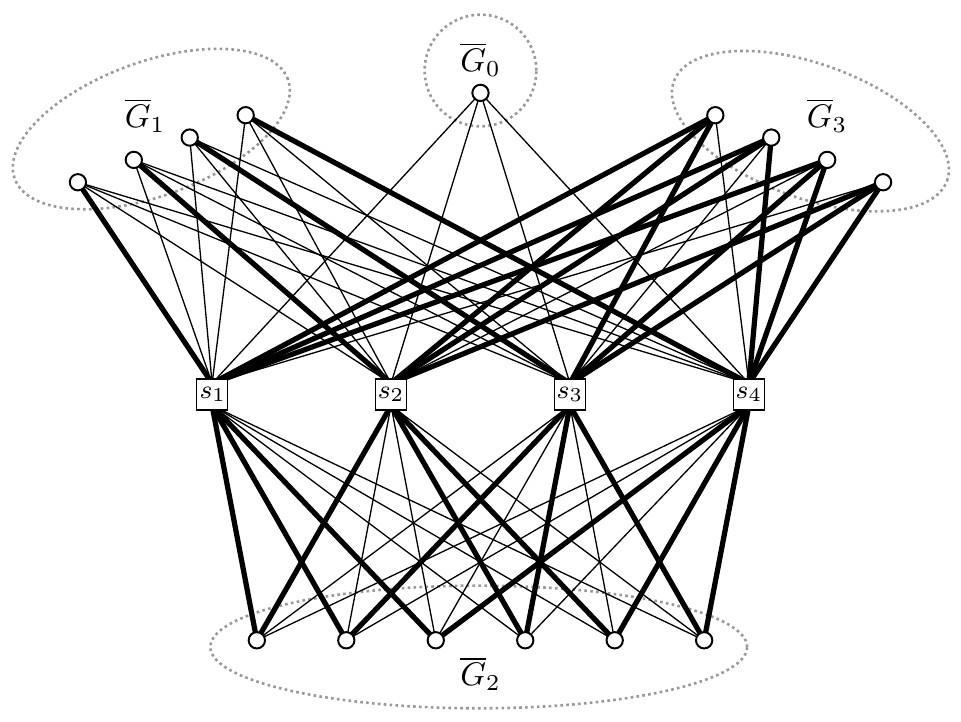
\includegraphics[width=0.6\textwidth]{images/k-server-advice.png}
    \caption{Konstruktion Graph für Beweis Advice-Komplexität von k-Server}
    \label{k-server-advice}
\end{figure}

\paragraph{Advice und Randomisierung}
Idee: Orakel muss zwar deterministisch sein, kann aber die Advice-Bits als die ``besten''
Zufallsbits wälen.

Wenn ein c-kompetitiver randomisierter OA existiert der $b(n)$ Zufallsbits liest,
so existiert auch ein c-kompetitiver OA mit Advice der $b(n)$ Advice-Bits liest, und vice versa.

Wenn \emph{kein} OA mit Advice existiert der $b(n)$ Advice-Bits liest,
so existiert auch \emph{kein} randomisierter OA der $b(n)$ Zufallsbits liest.

\paragraph{Satz (6.1)}
Sei $\Pi$ ein Online-Minimierungsproblem für das $m(n)$ verschiedene Instanzen der Länge $n$ existieren.
\footnote{Wir müssen die Anzahl der möglichen Eingaben einschränken.}
Sei $Rand$ ein randomisierter OA mit erwartetem kompetitiven Faktor $c$.

Dann existiert ein OA mit Advice der $((1 + \varepsilon) c)$-kompetitiv ist und Advice-Komplexität
$$\log \log (m(n))$$
hat. \footnote{Stark vereinfacht im Vergleich zum Skript.}
D.h. die Anzahl benötigter Advice-Bits hängt nur von der Anzahl Instanzen ab.

Umgekehrt: falls ein OA mit Advice mindestens mehr Advice-Bits braucht,
dann kann kein randomisierter OA existieren.

\newpage

\section{Online-Rucksackproblem}

\begin{takeaway}
    \item Online-Rucksackproblem
    \item Ansätze: deterministisch, mit Advice, randomisiert
    \item Untere Schranken für den (erwarteten) kompetitiven Faktor und die Advice-Komplexität
\end{takeaway}

\paragraph{Online-Rucksackproblem}
Eingabe $I=(w_1, ..., w_n)$, wobei wir vereinfachen mit \mbox{Gewicht = Wert}.
$w_i \in \R, 0 \leq w_i \leq 1$ (nicht $w_i \in \N$ wie bei Offline!).
In jedem Zeitschritt $i$ muss $A$ entscheiden ob er $w_i$ einpacken will.
Dies kann nicht aufgeschoben oder revidiert werden.

Zulässige Lösung: Menge von Indizes $S \subseteq \{1, ..., n\}$ so dass
$gain(A(I)) := \sum_{i \in S} w_i \leq 1$.
\\
Ziel: $gain(A(I))$ maximieren.


\subsection{Deterministisch}

\paragraph{Satz}
Jeder deterministische OA für das Rucksackproblem hat einen beliebig grossen (d.h schlechten)
kompetitiven Faktor.

\underline{Beweis:}
Schritt 1: Gegenspieler bietet Objekt $w$ mit Gewicht $\varepsilon > 0$ an.
Schritt 2: Falls $w$ akzeptiert, biete Objekt mit Gewicht 1 an. Falls $w$ verworfen, breche ab.
\\
$\implies$ kompetitiver Faktor von $\frac{1}{\varepsilon}$ bzw. von
$\frac{\varepsilon}{0}$/unendlich/undefiniert.

\vspace{5mm}

Trotzdem ist $Greedy$ auf bestimmte Klassen von Eingaben gut:

\paragraph{Satz}
Für jede Instanz mit Gewichten $\leq \beta$ ist $Greedy$ optimal oder erreicht einen Gewinn von $> 1-\beta$.

\underline{Beweis:}
Fallunterscheidung: Gesamtgewicht aller angebotenen Objekte $\leq 1$ (optimal), oder $> 1$ (dann
ist in $Greedy$'s Sack nur $< \beta$ Platz leer).

\paragraph{Satz}
Für jede Instanz mit $gain(Opt(I)) \leq \frac{1}{2}$ ist $Greedy$ optimal.

\underline{Beweis:}
Offensichtlich gilt $gain(Greedy(I)) \leq \frac{1}{2}$.
Falls $gain(Greedy(I)) < gain(Opt(I))$, dann ...
TODO
% Laut Skript: ... muss $Greedy$ ein Objekt mit Gewicht $> \frac{1}{2}$ verworfen haben.
% Mir ist nicht klar ob/warum dies gilt.
% Ich würde argumentieren es kann keine weiteren Objekte geben.
% Denn die mit >=1/2 hätte Opt direkt eingepackt,
% und die mit >1/2 hätte Opt auch eingepackt (und dafür alle eben noch eingepackten verworfen).


\subsection{Mit Advice}

\paragraph{Satz (Triviale untere Schranke)}
Es existiert ein optimaler OA mit Advice für das Rucksackproblem der $n$ Advice-Bits benutzt.

\underline{Beweis}: Left as an exercise to the reader.

\paragraph{Satz (Scharfe Schranke)}
Jeder optimale OA mit Advice für das Rucksackproblem muss mindestens $n-1$ Advice-Bits benutzen.

\underline{Beweis:}
Konstruiere Klasse von Instanzen:
$ I = (\frac{1}{2}, \frac{1}{4}, ... , \frac{1}{2^{n-1}}, w_b)$
wobei $ w_b = 1 - \sum_{i=1}^{n-1} b_i 2^{-i} $ für einen beliebigen Binärstring $b$ der Länge $n-1$.
Für $n=8$ z.B. führt $b=1101101$ zu
$$ w_b = 1 - \left( \frac{1}{2} + \frac{1}{4} + 0 + \frac{1}{16} + \frac{1}{32} + 0 + \frac{1}{128} \right) $$
Die eindeutige optimale Lösung hat Gewinn 1, und füllt mit den ersten $n-1$ Objekten die ``Lücken''
von $w_b$ auf.

Es gibt $2^{n-1}$ veschiedene Binärstrings der Länge $n-1$, d.h. es gibt ebenso viele Instanzen.
Ein optimaler OA mit Advice muss alle unterscheiden können, d.h. er braucht $n-1$ Advice-Bits.
\\
Mit weniger Bits verhält er sich auf zwei Instanzen gleich (Schubfachprinzip),
und kann nicht auf beide optimal sein.

\paragraph{Algorithmus: KPone}
Lese ein Advice-Bit. Es entscheidet zwischen: Greedy von Beginn an, oder Warten auf ein Objekt
mit Gewicht $> \frac{1}{2}$ und ab dann Greedy.

\paragraph{Satz}
Der OA mit Advice $KPone$ für das Rucksackproblem ist strikt 2-kompetitiv.

\underline{Beweis:}
\\
Fall 1: ein Objekt mit Gewicht $> \frac{1}{2}$ existiert. $KPone$ packt dieses ein,
$\implies gain(KPone(I)) > \frac{1}{2}$.
\\
Fall 2: Setze $\beta = 2$ und wende obigen Satz für det. OAs an
$\implies gain(KPone(I)) \geq 1 - \frac{1}{2} = \frac{1}{2}$ (oder optimal).

Dann gilt:
$$ \frac{gain(Opt(I))}{gain(KPone(I))} \leq \frac{1}{gain(KPone(I))} \leq \frac{1}{\frac{1}{2}} = 2 $$

\paragraph{Fazit}
Mit $n-1$ Advice-Bits sind wir optimal, mit 1 Advice-Bit bereits 2-kompetitiv.
Konstant mehr Bits helfen nicht.

Untere Schranke: kein OA mit $< \log_2 (n-1)$ Advice-Bits kann besser als $(2-\varepsilon)$-kompetitiv sein.
\footnote{Beweis ähnlich wie oben, via Konstruktion einer Klasse von Instanzen und Schubfachprinzip.}
\\
Obere Schranke: mit $\bigO(\log n)$ Advice-Bits kommen wir beliebig nah an die optimale Lösung heran.


\subsection{Randomisiert}

\paragraph{Motivation}
Ein Advice-Bit ist mächtig. Wie mächtig ist ein Zufallsbit?

\paragraph{Algorithmus: RKPone'}
Wie KPone, aber statt Advice-Bit nimmt er ein Zufallsbit.

\paragraph{Satz}
Der Barely-Random-Algorithmus $RKPone'$ ist strikt 4-kompetitiv im Erwartungswert.
Diese Schranke ist dicht (d.h. er kann nicht besser sein).

\paragraph{Algorithmus: RKPone}
Wähle u.a.r. einen deterministischen OA aus $strat(RKPone) = \{ Greedy_1, Greedy_2 \}$.
\\
$Greedy_1$ ist eine normale Greedy-Strategie.
\\
$Greedy_2$ simuliert $Greedy_1$, akzeptiert aber nichts. Sobald ein Objekt nicht mehr in $Greedy_1$s
Rucksack passt, akzeptiert $Greedy_2$ dieses und folgt von dann an einer Greedy-Strategie.

\paragraph{Satz}
Der Barely-Random-Algorithmus $RKPone$ ist strikt 2-kompetitiv im Erwartungswert.

\underline{Beweis:}

Fall 1: $\sum w_i \leq 1$ $\implies$ $gain(Greedy_1(I)) = gain(Opt(I)) \leq 1$ und $gain(Greedy_2(I))=0$ \\
$\implies$ erwartete Gewinn = $\frac{1}{2} \cdot gain(Opt(I))$

Fall 2: $\sum w_i \geq 1$. Dann ist der erwartete Gewinn:
$$ \frac{1}{2} gain(Greedy_1(I)) + \frac{1}{2} gain(Greedy_2(I))
= \frac{1}{2} \left( gain(Greedy_1(I)) + gain(Greedy_2(I)) \right) \geq \frac{1}{2} $$
wobei wir verwenden dass $gain(Greedy_1(I)) + gain(Greedy_2(I)) \geq 1$
(da $Greedy_2$ mindestens das Objekt akzeptiert mit dem $Greedy_1$ die Rucksackkapazität überschritten hätte).

\paragraph{Satz (Untere Schranke)}
Kein randomisierter OA für das Rucksackproblem ist besser als strikt 2-kompetitiv im Erwartungswert.

Intuitiv: ein Advice-Bit ist genauso mächtig wie beliebig viel Randomisierung.

\underline{Beweis:}
Betrachte die Klasse von Instanzen $\mathcal{I} = \{ I_1=(\varepsilon ), I_2=(\varepsilon , 1) \} $.
Sei $Rand$ ein randomisierter OA der $x_1$ mit Wahrscheinlichkeit $p$ akzeptiert.
\footnote{$p>0$ muss gelten da $Rand$ sonst auf $I_1$ einen erwarteten Gewinn von 0 hat.}

Für den kompetitive Faktor gilt:
$$
KF(I_1) = \frac{\varepsilon}{p \cdot \varepsilon + (1-p) \cdot 0} = \frac{1}{p} \qquad ; \qquad
KF(I_2) = \frac{1}{p \cdot \varepsilon + (1-p) \cdot 1} $$
Durch Gleichsetzen folgt $ p = \frac{1}{2 - \varepsilon} $, und durch Rückeinsetzen in $KF$ folgt
dass der kompetitive Faktor $\geq 2 - \varepsilon$ ist.

\newpage

\end{document}
